\chapter{Três Distribuições Fundamentais: Binomial, Gaussiana e Poisson}

\section{A Distribuição Binomial}

Um experimento \textbf{binário} só pode ter dois resultados possíveis, que podem ser interpretados como \textbf{sucesso} ou \textbf{falha}, como por exemplo o lançamento de uma moeda. Mesmo experimentos complexos com um maior número de resultados possíveis podem ser descritos como binários, quando se está simplesmente interessado na ocorrência de um evento específico $A$, ou sua não ocorrência, $A^\complement$. Por exemplo, o lançamento de um dado pode ser interpretado como um experimento binário se estivermos interessados na ocorrência do número seis, ou na ocorrência de qualquer outro número. É de fundamental importância em estatística determinar as propriedades dos experimentos binários, e a distribuição do número de sucessos quando o experimento é repetido várias vezes sob as mesmas condições experimentais. Uma variável aleatória binária é geralmente referida como \textbf{variável de Bernoulli}.

\subsection{Derivação da Distribuição Binomial}

Considere um experimento binário caracterizado por uma probabilidade de sucesso $p$ e, portanto, uma probabilidade de falha $q = 1 - p$. As probabilidades $p$ e $q$ são determinadas de acordo com a teoria da probabilidade e são assumidas como conhecidas para o experimento em questão. Quando o experimento é repetido $N$ vezes nas mesmas condições experimentais, é interessante calcular a probabilidade de obter $n$ sucessos em $N$ tentativas. A ordem em que os $n$ sucessos ocorrem não é relevante; por exemplo, considere lançar uma moeda quatro vezes e estar interessado na probabilidade de exatamente duas dessas jogadas mostrarem cara. O cálculo da probabilidade binomial segue estes passos:
\begin{enumerate}[noitemsep]
\item \textbf{Probabilidade de uma sequência ordenada}. A probabilidade de ter $n$ sucessos e, portanto, $N - n$ falhas ocorrendo em uma ordem específica é dada por:
\begin{equation}\label{3.1}
P(\text{sequência específica de $n$ sucessos}) = p^n \times q^{N-n}.
\end{equation}
Este resultado pode ser visto usando a propriedade de independência entre os $N$ eventos, de modo que as probabilidades individuais podem simplesmente ser multiplicadas.

\item  \textbf{Número de sequências ordenadas ou permutações}. Comece contando quantas sequências ordenadas existem que têm $n$ sucessos em $N$ tentativas. Para começar, cada uma das $N$ tentativas pode resultar no ``primeiro'' sucesso, e portanto existem $N$ possibilidades para qual tentativa será o primeiro sucesso. Continuando para o ``segundo'' sucesso, sobram apenas $N - 1$ possibilidades para qual tentativa será o segundo sucesso, e assim por diante. Este método de contagem de sequências rotula cada sucesso como primeiro, segundo, etc., e leva ao número de permutações de $n$ sucessos em $N$ tentativas:
\begin{equation}\label{3.2}
\text{Perm}(n, N) = N \cdot (N - 1) \cdot (N - n + 1) = \dfrac{N!}{(N - n)!}.
\end{equation}

\begin{exemplo}{}{}
Considere o caso de $n = 2$ sucessos em $N = 4$ tentativas. De acordo com a \autoref{3.2}, o número de permutações é $4!/(4-2)! = 4!/2! = 12$. As 12 sequências ordenadas que resultam em 2 sucessos em 4 tentativas estão listadas na \autoref{tab:3-1}. O símbolo $S_1$ denota o ``primeiro sucesso'' e $S_2$ o ``segundo sucesso''. Considere, por exemplo, as linhas 5 e 8: ambas representam a mesma situação em que as tentativas 2 e 3 resultam em sucesso. Na realidade, elas não são sequências diferentes, mas simplesmente um resultado do método de contagem de sequências ordenadas no tempo.

\begin{center}
	\begin{tabular}{|c|cccc|c|cccc|}
		\hline
		\multirow{2}{*}{Sequência} & \multicolumn{4}{c|}{Número de tentativas}                                        & \multirow{2}{*}{Sequência} & \multicolumn{4}{c|}{Número de tentativas}                                        \\ \cline{2-5} \cline{7-10} 
		& \multicolumn{1}{c|}{1} & \multicolumn{1}{c|}{2} & \multicolumn{1}{c|}{3} & 4     &                            & \multicolumn{1}{c|}{1} & \multicolumn{1}{c|}{2} & \multicolumn{1}{c|}{3} & 4     \\ \hline
		1                          & $S_1$                  & $S_2$                  & --                     & --    & 7                          & $S_2$                  & --                     & $S_1$                  & --    \\ \cline{1-1} \cline{6-6}
		2                          & $S_1$                  & --                     & $S_2$                  & --    & 8                          & --                     & $S_2$                  & $S_1$                  & --    \\ \cline{1-1} \cline{6-6}
		3                          & $S_1$                  & --                     & --                     & $S_2$ & 9                          & --                     & --                     & $S_1$                  & $S_2$ \\ \cline{1-1} \cline{6-6}
		4                          & $S_2$                  & $S_1$                  & --                     & --    & 10                         & $S_2$                  & -                      & --                     & $S_1$ \\ \cline{1-1} \cline{6-6}
		5                          & --                     & $S_1$                  & $S_2$                  & --    & 11                         & --                     & $S_2$                  & --                     & $S_1$ \\ \cline{1-1} \cline{6-6}
		6                          & --                     & $S_1$                  & --                     & $S_2$ & 12                         & --                     & --                     & $S_2$                  & $S_1$ \\ \hline
	\end{tabular}
	\captionof{table}{Ilustração das permutações (sequências ordenadas) de 2 sucessos em 4 tentativas}
	\label{tab:3-1}
\end{center}

\end{exemplo}

\item \textbf{Número de sequências não ordenadas ou combinações}. Como fica claro a partir do exemplo anterior, o número de permutações não é exatamente o número procurado, uma vez que não importa qual sucesso é rotulado como primeiro, segundo, etc. De acordo com a \autoref{3.2}, no caso de $n = N$, há $n!$ maneiras de ordenar $n$ sucessos entre si. Portanto, o número de permutações (ordenadas no tempo) precisa ser dividido por $n!$ para evitar a contagem dupla de sequências equivalentes. Fica claro, portanto, que o número de \textbf{combinações} de $n$ sucessos em $N$ tentativas é:
\begin{equation}\label{3.3}
C(n, N) = \dfrac{\text{Perm}(n, N)}{n!} = \dfrac{N!}{n!(N-n)!} = \binom{N}{n}.
\end{equation}
O número de combinações é o número de sequências possíveis de $n$ sucessos em $N$ tentativas. Esse número, é chamado de \textbf{coeficiente binomial} e é indicado pelo símbolo entre parênteses. O coeficiente binomial é usado na expansão binomial:
\begin{equation}\label{3.4}
(p + q)^N = \sum_{n=0}^{N} \binom{N}{n} p^n q^{N-n}.
\end{equation}

\begin{exemplo}{}{}
Continue a considerar o caso de 2 sucessos em 4 tentativas. Existem $2! = 2$ maneiras de ordenar os 2 sucessos entre si (ou um ou o outro é o primeiro sucesso). Portanto, o número de combinações de 2 sucessos em 4 tentativas é $4!/[2!(4-2)!] = 6$, e não 12. Conforme indicado acima, de fato, cada sequência tinha sua sequência ``gêmea'' listada separadamente, e a \autoref{3.3} conta corretamente apenas sequências diferentes.
\end{exemplo}
\end{enumerate}

De acordo com os resultados obtidos acima, o que resta a ser feito é usar a probabilidade de cada sequência \eqref{3.1} e multiplicá-la pelo número de combinações na \autoref{3.3} para obter a probabilidade geral de ter $n$ sucessos em $N$ tentativas. Isso leva à função massa de probabilidade (FMP):
\begin{equation}\label{3.5}
P_N(n) = \binom{N}{n} p^n q^{N-n}, \quad n = 0, \ldots, N,
\end{equation}
conhecida como a \textbf{distribuição binomial}. Esta distribuição descreve a probabilidade de $n$ sucessos em $N$ tentativas de um experimento binário com probabilidade de sucesso $p$. A \autoref{3.4} mostra que a distribuição binomial é devidamente normalizada. Exemplos da distribuição binomial são mostrados na \autoref{fig:3-1}.

\begin{SCfigure}[\sidecaptionrelwidth][ht!]
	\centering
	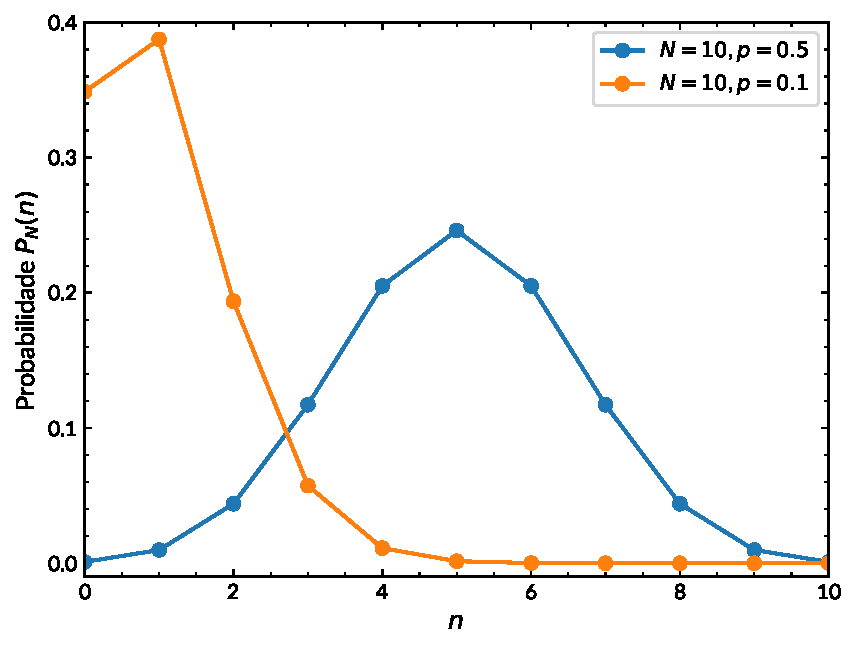
\includegraphics[width=0.7\linewidth]{Figuras/3-1.pdf}
	\caption{Distribuições binomiais de exemplo para $N = 10$ e $p = 0.5$, $p = 0.1$. A função é definida apenas para inteiros não negativos $0 \leq n \leq N$.}
	\label{fig:3-1}
\end{SCfigure}

\subsection{Momentos da Distribuição Binomial}

Os momentos de primeira e segunda ordem de uma variável $X$ distribuída binominalmente são dados por:
\begin{subequations}\label{3.6}
\begin{align}
\mathbb{E}[X] &= \mu = pN \\
\mathbb{E}[X^2] &= \mu^2 + pqN 
\end{align}
\end{subequations}
Vamos provar essas equações começando pela média,
\begin{equation*}
\mathbb{E}[X] = \sum_{n=0}^{N} n P_N(n) = \sum_{n=0}^{N} \binom{N}{n} n p^n q^{N-n} = \sum_{n=0}^{N}  \binom{N}{n} \left[p \dfrac{\partial}{\partial p}\right]p^n q^{N-n};
\end{equation*}
O operador linear $p\frac{\partial}{\partial p}$ pode ser aplicado a toda a soma, levando a (considere a substituição da \autoref{3.4} aqui):
\begin{equation*}
\mathbb{E}[X] = p \dfrac{\partial}{\partial p} \sum_{n=0}^{N} \binom{N}{n} p^n q^{N-n} = p \dfrac{\partial}{\partial p} (p + q)^N = pN(p + q)^{N-1} = pN,
\end{equation*}
onde o último passo se deve ao fato de que $p + q = 1$. A derivação para o momento $\mathbb{E}[X^2]$ é similar:
\begin{equation*}
\mathbb{E}[X^2] = \sum_{n=0}^{N} n^2 P_N(n) = \sum_{n=0}^{N} \binom{N}{n} n^2p^n q^{N-n}.
\end{equation*}
Observe que, se $np^n = p\frac{\partial}{\partial p}p^n$, a seguinte expressão é válida:
\begin{equation*}
n^2p^n = p\frac{\partial}{\partial p} \left(np^n\right) = \left(p\frac{\partial}{\partial p}\right)\left(p\frac{\partial}{\partial p}\right)p^n = \left(p\frac{\partial}{\partial p}\right)^2p^n.
\end{equation*}
Assim, 
\begin{align*}
\mathbb{E}[X^2] = \sum_{n=0}^{N} \binom{N}{n} \left(p\frac{\partial}{\partial p}\right)^2 p^nq^{N-n} =  \left(p\frac{\partial}{\partial p}\right)^2 (p + q)^N = p\frac{\partial}{\partial p} \left[pN (p + q)^{N -1}\right].
\end{align*}
Desenvolvendo, 
\begin{align*}
\mathbb{E}[X^2] &= p\left[N(p + q)^{N -1} + pN(N - 1)(p + q)^{N - 2}\right] = pN + (pN)^2 - p^2N \\
&= (pN)^2 + pN(1 - p) = (pN)^2 + pqN,
\end{align*}
onde novamente usamos o fato de que $p + q = 1$. 

Segue-se que a variância da distribuição binomial é dada por:
\begin{equation}\label{3.7}
\sigma^2 = \mathbb{E}[X^2] - \mathbb{E}[X]^2 = (pN)^2 + pqN - (pN)^2 = pqN.
\end{equation}
As equações \eqref{3.6} e \eqref{3.7} descrevem as características mais importantes da distribuição binomial, mostradas na \autoref{fig:3-1} para o caso de $N = 10$. A média é naturalmente dada pelo produto do número de tentativas $N$ e a probabilidade de sucesso \(p\) em cada uma das tentativas.

\begin{exemplo}{}{}
Uma companhia aérea sabe que 5\% das pessoas que fazem reservas não aparecerão no portão de embarque. Para um voo com capacidade para 50 passageiros, a companhia vendeu 52 passagens e quer determinar a probabilidade de que haverá um assento disponível para cada passageiro que aparecer. Utilizando a distribuição binomial, onde cada passageiro tem uma probabilidade $p = 0.95$ de aparecer, queremos calcular a probabilidade de que no máximo 50 dos 52 passageiros compareçam ($P(X \leq 50)$). Definindo $X$ como a variável aleatória que representa o número de passageiros que aparecem, temos $X \sim \text{Binomial}(N = 52, p = 0.95)$. A probabilidade desejada é dada por:
\begin{equation*}
P(X \leq 50) = 1 - P(X = 52) - P(X = 51),
\end{equation*}
onde, usando a fórmula da distribuição binomial \eqref{3.5},
\begin{align*}
P(X = 52) &= \binom{52}{52} (0.95)^{52} (0.05)^0 = (0.95)^{52}\\
P(X = 51) &= \binom{52}{51} (0.95)^{51} (0.05)^1 = 52 \cdot (0.95)^{51} \cdot 0.05.
\end{align*}
Calculando esses valores, obtemos:
\begin{equation*}
P(X \leq 50) = 1 - (0.95)^{52} - 52 \cdot (0.95)^{51} \cdot 0.05 \approx 0.741.
\end{equation*}
Assim, a probabilidade de que haverá um assento disponível para cada passageiro que aparecer é aproximadamente 74.1\%. Consequentemente, a companhia aérea está assumindo um risco de 25.9\% de ter um voo com \textit{overbooking}.
\end{exemplo}

\section{A Distribuição Gaussiana}

A distribuição Gaussiana, frequentemente referida como \textbf{distribuição normal}, desempenha um papel especial na estatística. Uma variável aleatória contínua $X$ é dita ter uma distribuição Gaussiana se sua função densidade de probabilidade (FDP) for
\begin{equation}
f(x) = \dfrac{1}{\sqrt{2\pi \sigma^2}} \exp\left[-\dfrac{(x-\mu)^2}{2\sigma^2}\right]
\end{equation}
A função de distribuição é definida para todos os valores reais, e sua forma é determinada pelos dois parâmetros $\mu$ e $\sigma^2$, que também representam a média e a variância da variável aleatória (veja a \autoref{fig:3-2}). Uma Gaussiana com parâmetros $\mu$ e $\sigma^2$ é frequentemente referida como $\mathcal{N}(\mu, \sigma^2)$. É útil mostrar que a distribuição Gaussiana pode ser considerada um caso especial da distribuição binomial, no caso de um grande número de experimentos realizados.

\begin{SCfigure}[\sidecaptionrelwidth][ht!]
	\centering
	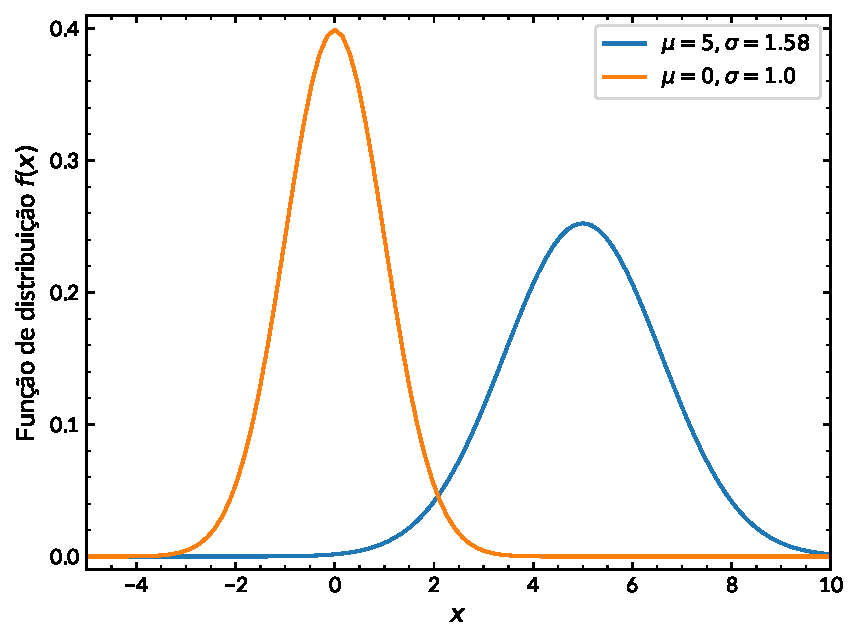
\includegraphics[width=0.7\linewidth]{Figuras/3-2.pdf}
	\caption{Distribuições Gaussianas para valores selecionados da média e variância. A curva Gaussiana em azul tem a mesma média e variância que uma distribuição binomial com $N = 10$ e $p = 0.5$ (mostrada na \autoref{fig:3-1}).}
	\label{fig:3-2}
\end{SCfigure}
